\begin{figure}[!t]
\begin{tabular}{|p{.98\linewidth}|}\hline
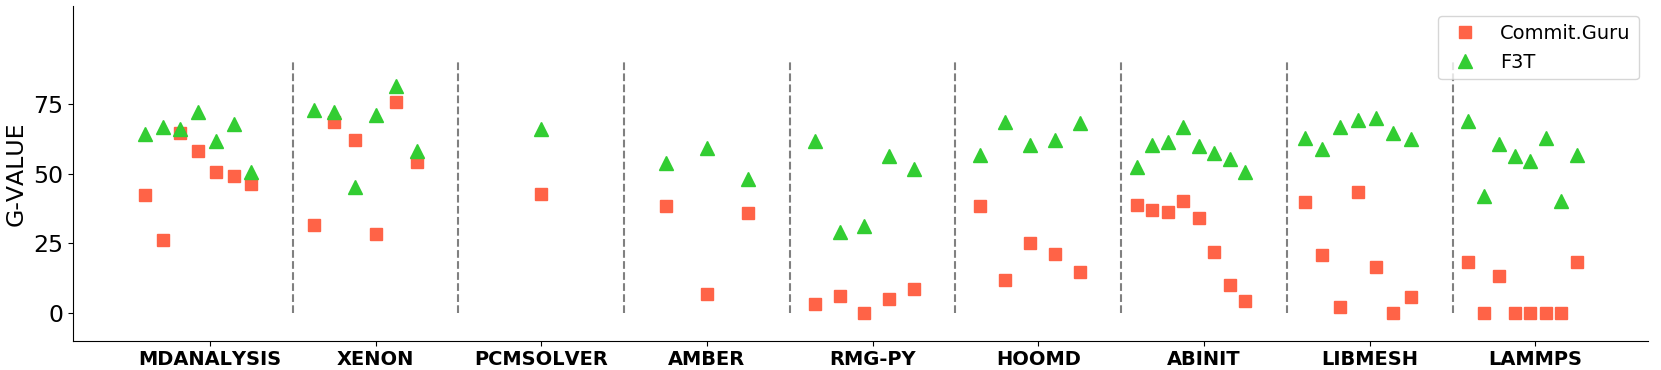
\includegraphics[width=\linewidth]{fig/rq3_1.png}
\small
\bi
\item Data
from 9 computational science projects
was extracted from on-line repositories.
\item
A Random Forest classifier was trained on release {\em r-1} to predict
for ``is buggy'' in the next release {\em r}.
\item
Y-axis shows
 ``G-values'' (harmonic mean of recall and  1 - false alarm) so {\em larger} means {\em better} defect predictors.
\item
Results shown as \textcolor{red}{\bf RED} squares come from standard empirical SE methods (using the Commit.Guru tool~\cite{commitguru}) that uses standard small set of keywords on the commit message 
%and (2) Logistic Regression learner 
to decide if a commit is ``buggy'' or not). As witnessed by the low red values, those
standard methods performed very badly.
\item
The \textcolor{ForestGreen}{\bf GREEN} triangles show
much better results from {\em active learning}~\cite{settles2012active}. It specifically built a specialized language model for these commit logs from computational science software to retrieve more ``accurate'' dependent variable for the data. 
%Here, an incrementally modified text miner (a support vector) presents to a human the  example it thinks is mostly likely to be buggy. Humans label this example as  ``buggy'' or ``non-buggy''. The SVM then retrains using this new example. 
\ei
\\\hline
\end{tabular}
\caption{
Computational science defect prediction patterns found in 36,110  commit  messages.
Standard SE methods (shown in \textcolor{red}{\bf RED})  failed  {\em until} we 
actively learned
a new language model that was especially tuned to the language of computational scientists (see the \textcolor{ForestGreen}{\bf GREEN} results).
}\label{fig:redgreen}
\end{figure}   
